
\section{Discusión}

En este último apartado, tomando como referencia los NACA 4-digit, se examina el comportamiento del $\alpha_{l0}$ y el $C_{m0}$ en función de la posición de máxima combadura $\left( p \right)$ y el valor de esta $\left( f \right)$.

Se aplica el DVM a perfiles con $f$ en el rango $0$--$0.06$, en incrementos de $0.01$ y $p$ de $0.1$--$0.6$ en incrementos de $0.1$. Para cada par $\left( f, p \right)$, se calculan el $C_l$ y el $C_{m0}$ en un rango lineal $\alpha_{1} = -10\degrees$ a $\alpha_{2} = 10\degrees$. Denotando $C_{li} = C_l\left( \alpha_i \right)$, el ángulo de sustentación nula se determina a partir de
\begin{equation}
    \alpha_{l0} = \frac{C_{l2} \alpha_1 - C_{l1} \alpha_2}{C_{l2} - C_{l1}}
\end{equation}
El $C_{m0}$ se calcula como el promedio en el rango lineal de $C_l$ elegido.

En la figura \ref{fig:discussion_alpha_l0} se representa el ángulo de sustentación nula en función de la posición de máxima combadura para distintas combaduras máximas. Lo propio con el coeficiente de momento libre se muestra en la figura \ref{fig:discussion_cm0}.

En la figura \ref{fig:discussion_cm0} se representa el coeficiente de momento libre en función de la posición de máxima combadura para distintas combaduras máximas. Lo propio con el ángulo de sustentación nula se muestra en la figura \ref{fig:discussion_cm0}.

\begin{figure}[ht] 
    \centering
    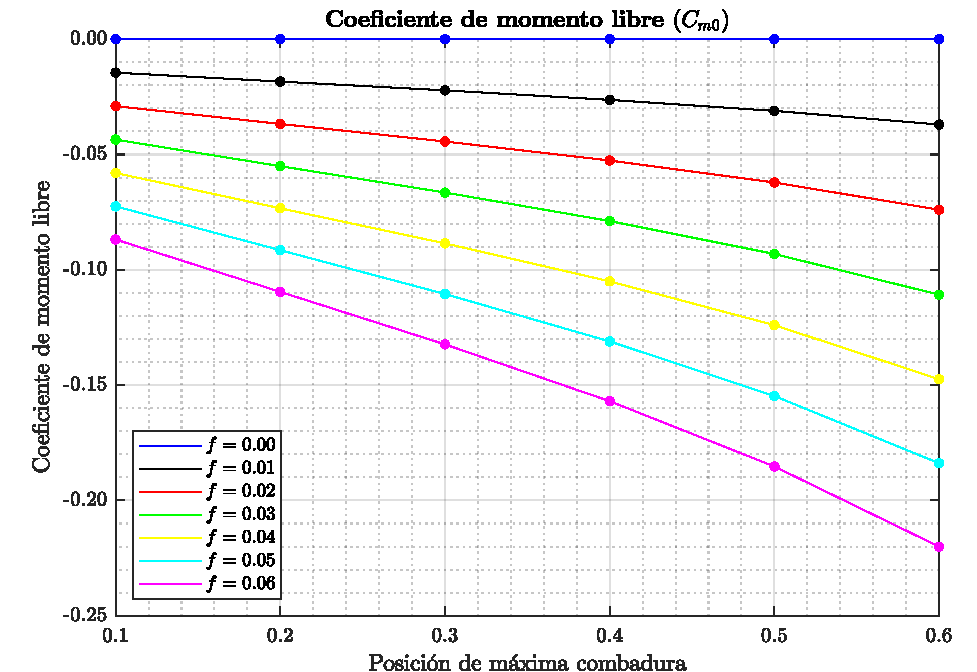
\includegraphics[width=\linewidth]{imagenes/discusion/discussion_cm0.pdf}
    \caption{Coeficiente de momento libre $\left( C_{m0} \right)$ en función de la posición de máxima combadura $\left( p \right)$, para distintas combaduras máximas $\left( f \right)$.}
    \label{fig:discussion_cm0}
\end{figure}

\begin{figure}[ht] 
    \centering
    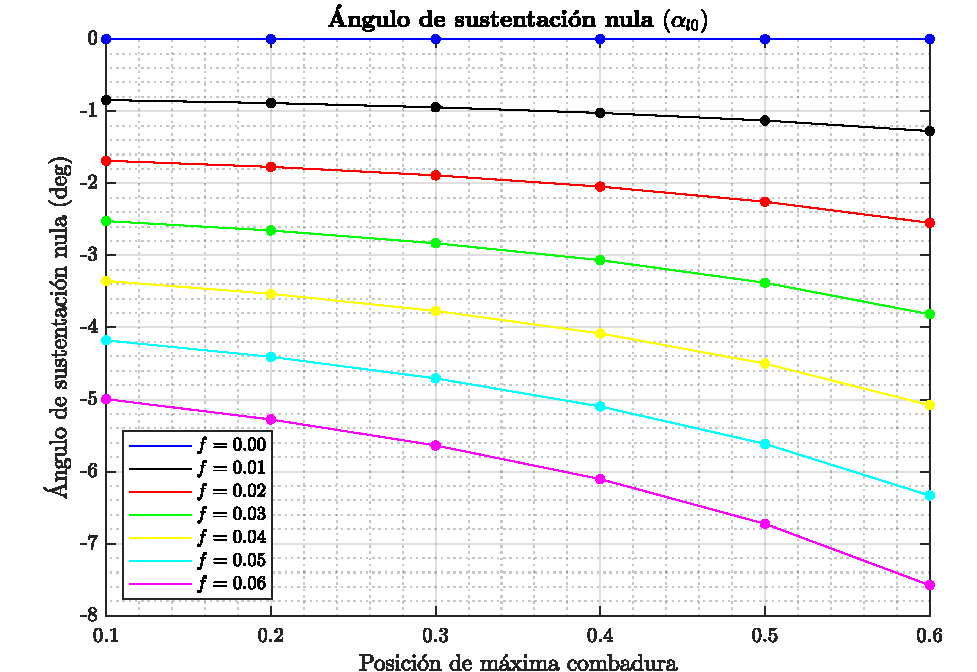
\includegraphics[width=\linewidth]{imagenes/discusion/discussion_alpha_l0.pdf}
    \caption{Ángulo de sustentación nula $\left( \alpha_{l0} \right)$ en función de la posición de máxima combadura $\left( p \right)$, para distintas combaduras máximas $\left( f \right)$.}
    \label{fig:discussion_alpha_l0}
\end{figure}

Se aprecia que el $C_{m0}$ disminuye cuando $f$ y $p$ aumentan. Tal como predice la TAT, cuando $f = 0$, \ie, un perfil simétrico, el $C_{m0}$ es nulo. A medida que la posición de máxima combadura se desplaza hacia el borde de salida, la curvatura en esta zona aumenta. Según el modelo de flujo potencial usado por la TAT \cite{ortega}, el flujo se mantiene adherido. Cuando el flujo se curva este se acelera, intercambiando energía de presión por energía cinética. Consecuentemente, la presión local disminuye, \ie, el coeficiente de presión $\left( C_p \right)$ disminuye. Aparece así la sustentación $\left( L \right)$, debida a la diferencia de presiones. Al estar desplazada hacia el borde de salida, el brazo de palanca de $L$ aumenta, volviendo más negativo el momento libre. Esto se justifica con resultados experimentales. Según \cite{nasa_cp}, para el perfil NACA 6716, la recuperación de presión en el extradós es abrupta, \ie, $d C_p / d x$ es importante hasta llegar a la posición de máxima combadura. En esta zona la recuperación de presión se reduce. 

De igual forma sucede con el ángulo de sustentación nula. Conforme $f$ y $p$ aumentan, el $\alpha_{l0}$ disminuye, \ie, su módulo aumenta. De nuevo, para perfil simétrico, se tiene $\alpha_{l0} = 0$, en concordancia con la TAT. Como en el caso del momento libre, a mayor $f$ y $p$, la carga aerodinámica sobre la zona del borde de salida es mayor para todo ángulo de ataque. En consecuencia, el ángulo de ataque de sustentación nula se incrementa en valor absoluto.

En ambos casos se ha visto que un aumento de $f$ y $p$ comporta un aumento en los valores absolutos de $\alpha_{l0}$ y $C_{m0}$. Dentro de unos márgenes razonables, aumentar el ángulo de sustentación nula resulta beneficioso, pues la sustentación será mayor para ángulos de ataques menores. No obstante el ángulo de entrada en pérdida $\left( \alpha_\text{stall} \right)$ disminuye. Asimismo, el $C_{m0}$ disminuye, pudiendo afectar a la estabilidad de la aeronave. Por lo tanto, desde el diseño debe encontrarse el equilibrio adecuado entre $\alpha_{l0}$ y $C_{m0}$.
